\documentclass[11pt]{article}

\usepackage{filecontents}
\begin{filecontents}{\jobname.bib}
@article{rabosky2014bammtools,
  title={BAMMtools: an R package for the analysis of evolutionary dynamics on phylogenetic trees},
  author={Rabosky, Daniel L and Grundler, Michael and Anderson, Carlos and Shi, Jeff J and Brown, Joseph W and Huang, Huateng and Larson, Joanna G and others},
  journal={Methods in Ecology and Evolution},
  volume={5},
  number={7},
  pages={701--707},
  year={2014},
  publisher={Wiley Online Library}
}
@article{rabosky2014automatic,
  title={Automatic detection of key innovations, rate shifts, and diversity-dependence on phylogenetic trees},
  author={Rabosky, Daniel L},
  journal={PloS one},
  volume={9},
  number={2},
  pages={e89543},
  year={2014},
  publisher={Public Library of Science}
}
@article{beaulieu2015detecting,
  title={Detecting hidden diversification shifts in models of trait-dependent speciation and extinction},
  author={Beaulieu, Jeremy M and O'Meara, Brian C},
  journal={bioRxiv},
  pages={016386},
  year={2015},
  publisher={Cold Spring Harbor Labs Journals}
}
@article{rabosky2015model,
  title={Model inadequacy and mistaken inferences of trait-dependent speciation},
  author={Rabosky, Daniel L and Goldberg, Emma E},
  journal={Systematic Biology},
  volume={64},
  number={2},
  pages={340--355},
  year={2015},
  publisher={Oxford University Press}
}
@article{goldberg2011phylogenetic,
  title={Phylogenetic inference of reciprocal effects between geographic range evolution and diversification},
  author={Goldberg, Emma E and Lancaster, Lesley T and Ree, Richard H},
  journal={Systematic Biology},
  volume={60},
  number={4},
  pages={451--465},
  year={2011},
  publisher={Oxford University Press}
}
@article{fitzjohn2012diversitree,
  title={Diversitree: comparative phylogenetic analyses of diversification in R},
  author={FitzJohn, Richard G},
  journal={Methods in Ecology and Evolution},
  volume={3},
  number={6},
  pages={1084--1092},
  year={2012},
  publisher={Wiley Online Library}
}
@article{maddison2007estimating,
  title={Estimating a binary character's effect on speciation and extinction},
  author={Maddison, Wayne P and Midford, Peter E and Otto, Sarah P},
  journal={Systematic biology},
  volume={56},
  number={5},
  pages={701--710},
  year={2007},
  publisher={Oxford University Press}
}
@article{matzke2014model,
  title={Model selection in historical biogeography reveals that founder-event speciation is a crucial process in island clades},
  author={Matzke, Nicholas J},
  journal={Systematic Biology},
  volume={63},
  number={6},
  pages={951--970},
  year={2014},
  publisher={Oxford University Press}
}
\end{filecontents}

\usepackage{natbib}
\usepackage{adjustbox}
\usepackage{amsmath}
\usepackage[font=footnotesize]{caption}
\usepackage[dvipsnames]{xcolor}
\usepackage{geometry}
  \geometry{margin=1in}
\usepackage{framed}
\usepackage[breaklinks]{hyperref}
\usepackage{minibox}
\usepackage[compact]{titlesec}
\usepackage{listings,color}
\usepackage{float}

\definecolor{verbgray}{gray}{0.9}

\lstnewenvironment{code}{%
  \lstset{backgroundcolor=\color{verbgray},
  frame=single,
  framerule=0pt,
  basicstyle=\ttfamily\scriptsize,
  columns=fullflexible}}{}

\definecolor{shadecolor}{rgb}{.9, .9, .9}

\graphicspath{ {./figures/} }




\begin{document}


\noindent
\large
\begin{minipage}{0.5\textwidth}
\begin{flushleft} 
IB200, Spring 2016
\end{flushleft}
\end{minipage}
\begin{minipage}{0.5\textwidth}
\begin{flushright} 
\textit{University of California, Berkeley}
\end{flushright}
\end{minipage}

\vspace{0.5cm}


\begin{center}
\Large \textbf{Lab 13:} \\
Estimating Diversification Rates: \\
Heterogenous and Character Dependent Processes \\
\normalsize
\textit{By Will Freyman} \\
\end{center}

\vspace{0.5cm}

\section{Before you begin}

Today's lab will use R and the software BAMM.
Please install R: \\
\url{https://www.r-project.org/} \\
Please install BAMM: \\
\url{http://bamm-project.org/}

\section{Introduction to heterogenous birth-death processes}

In labs 6 and 11 we used birth-death processes
as tree priors in Bayesian analyses.
These were birth-death processes with constant
speciation and extinction rates, and so
were homogenous diversification processes.
In this lab we'll look at heterogenous processes
in which the rates of diversification change 
over the tree.
The changes in diversification rates could be
caused by a change in a character state 
(e.g. a key innovation)
or they could be due to some other 
dynamic such as climate change or the availability of new niches.

\section{Character dependent birth-death processes}

In the first exercise we'll use the \textbf{binary-state speciation and extinction} \citep[BiSSE;][]{maddison2007estimating} 
model using the R package \textbf{diversitree} \citep{fitzjohn2012diversitree}.
BiSSE models the evolution of a binary character and a birth-death process jointly,
and uses a separate set of speciation and extinction rates
for each state of the character (see Figure 1).  
Under BiSSE, the diversification process is dependent
on the character's state.

\begin{figure}[H]
\centering
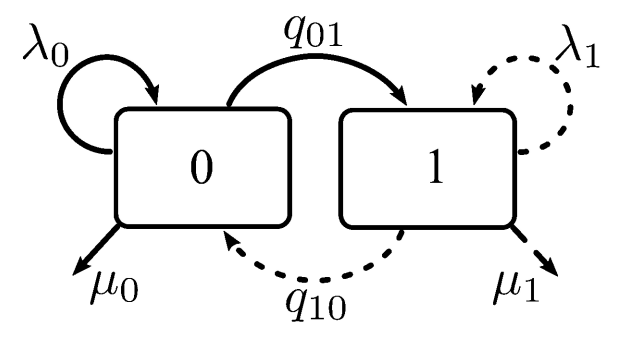
\includegraphics[width=0.4\textwidth]{bisse.png}
\caption{
States and transitions in the BiSSE model. BiSSE has 6 rate parameters:
speciation ($\lambda$) and extinction ($\mu$) for character states $0$ and $1$
and transition rates ($q$) for changing state.
Image from \protect\citet{goldberg2011phylogenetic}.}
\end{figure}



\subsection{Install and setup diversitree}

Start up R and install the diversitree package:
\begin{code}
install.packages("diversitree")
\end{code}
Now lets load the package:
\begin{code}
library(diversitree)
\end{code}

\subsection{Simulate constant rate birth-death process}

Let's first simulate a constant rate birth-death process.
We'll simulate a tree where speciation $\lambda$ is $0.1$
and extinction $\mu$ is $0.03$.
We'll save our diversification rates in a vector, and simulate the tree
for 30 time units:
\begin{code}
div_rates = c(0.2, 0.03)
tree = tree.bd( div_rates, max.t=30.0 )
\end{code}
Let's plot the tree:
\begin{code}
plot(tree)
axisPhylo()
\end{code}
Try simulating and plotting a few trees with different
values of $\lambda$ and $\mu$.

\subsection{Simulate an independent binary character over the tree}

Now let's simulate a character evolving neutrally over
the tree. During the evolution of this character the tree
is fixed -- the state of the character is independent of
the diversification process.
We'll use the \textbf{Mk2} model which simply
allows for two separate transition rates between
character states, $q_{01}$ and $q_{10}$.
\begin{code}
char_rates = c(.1, .2)
character = sim.character(tree, char_rates, x0=0, model="mk2")
\end{code}
Let's plot our character so we can see the way it evolved
over the tree:
\begin{code}
plot(tree, show.tip.label=FALSE)
axisPhylo()
colors=c("lightblue", "blue")
tiplabels(col=colors[character+1], pch=19, adj=1)
nodelabels(col=colors[attr(character, "node.state")+1], pch=19)
\end{code}
Try simulating and plotting with different 
values of $q_{01}$ and $q_{10}$.

\subsection{Simulate under BiSSE}

Now we will simulate a tree and a binary character jointly
using BiSSE. 
Whenever the character is in state 1 the speciation
rate will be triple that of state 0.
First set up our rates vector in the order
$\lambda_0$, 
$\lambda_1$,
$\mu_0$,
$\mu_1$,
$q_{01}$,
$q_{10}$.
We'll also set the random number generator seed to 13 so
that we all get the same results.
\begin{code}
set.seed(13)
rates =  c(0.1, 0.3, 0.03, 0.03, 0.01, 0.01)
\end{code}
Now let's simulate our tree and character
and then plot it:
\begin{code}
tree = tree.bisse(rates, max.t=30, x0=0)
plot(history.from.sim.discrete(tree, 0:1), tree, col=colors, show.tip.label=FALSE)
\end{code}
You should see that at the base of the
tree the root state is 0 (light blue)
and it diversifies at a medium rate.
At about 17 time units ago one lineage transitions to state 1 (dark blue)
and undergoes a rapid radiation (Figure 2).

\begin{figure}[H]
\centering
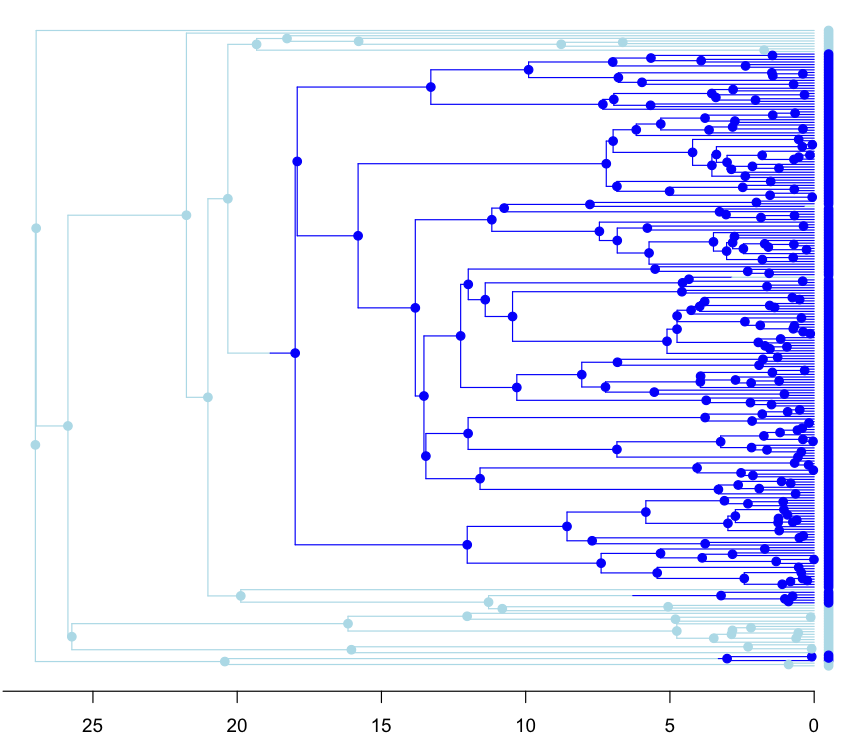
\includegraphics[width=0.6\textwidth]{sim.png}
\caption{Tree and binary character simulated under BiSSE. State 1 (dark blue)
has a speciatian rate three times that of state 0 (light blue).}
\end{figure}

\subsection{Testing for character dependent diversification}

We know the tree and character shown in Figure 2
evolved jointly under a BiSSE process;
the diversification process was dependent on the character.
However, in an actual empirical study usually all we have is a tree 
and the observed tip states.
How do we test for character dependent diversification?
Let's treat our simulated tree and tip data as if this was an empirical study
and see if we can successfully detect character dependent diversification.

First, let's fit a BiSSE model to the simulated data.
Since the diversification rate is dependent on the character state, 
the BiSSE likelihood function takes both the tree and the tip data:
\begin{code}
bisse_lik = make.bisse(tree, tree$tip.state)
\end{code}
We'll find the maximum likelihood estimate
for all parameters. We use a helper function to find
starting values of the parameters for the search heuristic.
\begin{code}
p = starting.point.bisse(tree)
fit_bisse = find.mle(bisse_lik, p)
\end{code}
What were the parameter estimates and log-likelihood?
\begin{code}
coef(fit_bisse)
fit_bisse$lnLik
\end{code}

Ok, now let's estimate diversification rates under
a constant rate model, where the diversification
process is independent of the character states. 
We'll use the same BiSSE likelihood function as above,
but constrain the diversification rates to be equal
in both character states:
\begin{code}
constant_lik = constrain(bisse_lik, lambda0 ~ lambda1, mu0 ~ mu1)
\end{code}
Again, find the maximum likelihood estimates of our parameters: 
\begin{code}
fit_constant = find.mle(constant_lik, p)
coef(fit_constant)
fit_constant$lnLik
\end{code}

Now let's use AIC to select the best model:
\begin{code}
AIC(fit_constant, fit_bisse)
\end{code}

\begin{framed}
\noindent
\textbf{Question 1:} \\
\begin{enumerate}
\item Which model did the AIC select? Can we successfully test for character dependent diversification?
\item Compare the estimated parameter values to the true values
    you used to simulate the data. How close were the speciation rates?
    What about the extinction rates?
\end{enumerate}
\end{framed}

\subsection{Extensions and caveats}

After the groundbreaking \citet{maddison2007estimating} introduced BiSSE,
an entire class of models were built upon it. 
These models have provided an exciting new quantitative framework to
test macroevolutionary patterns/processes such as adaptive radiations
and other ecological and geographic factors that affect the shape of the tree of life.
They include
MuSSE (Multiple State Speciation and Extinction), 
QuaSSE (Quantitative State Speciation and Extinction),
GeoSSE (Geographic State Speciation and Extinction),
and BiSSE-ness (BiSSE-Node Enhanced State Shift).
All these models are implemented in the excellent \textbf{diversitree}
R package.

However, these models have been found to be prone
to high Type 1 error rates, where characters
that evolved independent of the diversification process
are inferred to have statistically significant associations 
with diversification rates; 
the diversification process is erroneously inferred to be character dependent 
\citep{rabosky2015model}.
Novel extensions of these models that deal with these problems include the HiSSE (Hidden State Speciation and Extinction)
model, in which an unobserved ``hidden'' character is allowed to affects the diversification rates instead of the observed character \citep{beaulieu2015detecting}.
If you plan to use BiSSE or other similar models, be sure to test for false positives!

Run this code and then answer Question 2. 
It might take 5 to 10 minutes, so you may want to
go on to the next section while you wait.
\begin{code}
fp = 0
n = 20
char_rates = c(.1, .2)
for (i in 1:n) {
    print(paste("Beginning replicate", i, "out of", n))
    ind_character = sim.character(tree, char_rates, x0=0, model="mk2")
    dep_bisse_lik = make.bisse(tree, ind_character)
    fit_dep_bisse = find.mle(dep_bisse_lik, p)
    ind_constant_lik = constrain(dep_bisse_lik, lambda0 ~ lambda1, mu0 ~ mu1)
    fit_ind_constant = find.mle(ind_constant_lik, p)
    aic_results = AIC(fit_ind_constant, fit_dep_bisse)
    if (aic_results$AIC[[2]] < aic_results$AIC[[1]])
        fp = fp + 1
}
fp/n
\end{code}

\begin{framed}
\noindent
\textbf{Question 2:} \\
\begin{enumerate}
\item What did this code do? Describe what was being tested and how.
    All the major functions were described above.
\item What were the results? Put the results into context; what do
    they mean for analyses using BiSSE type models?
\end{enumerate}
\end{framed}

\begin{figure}[H]
\centering
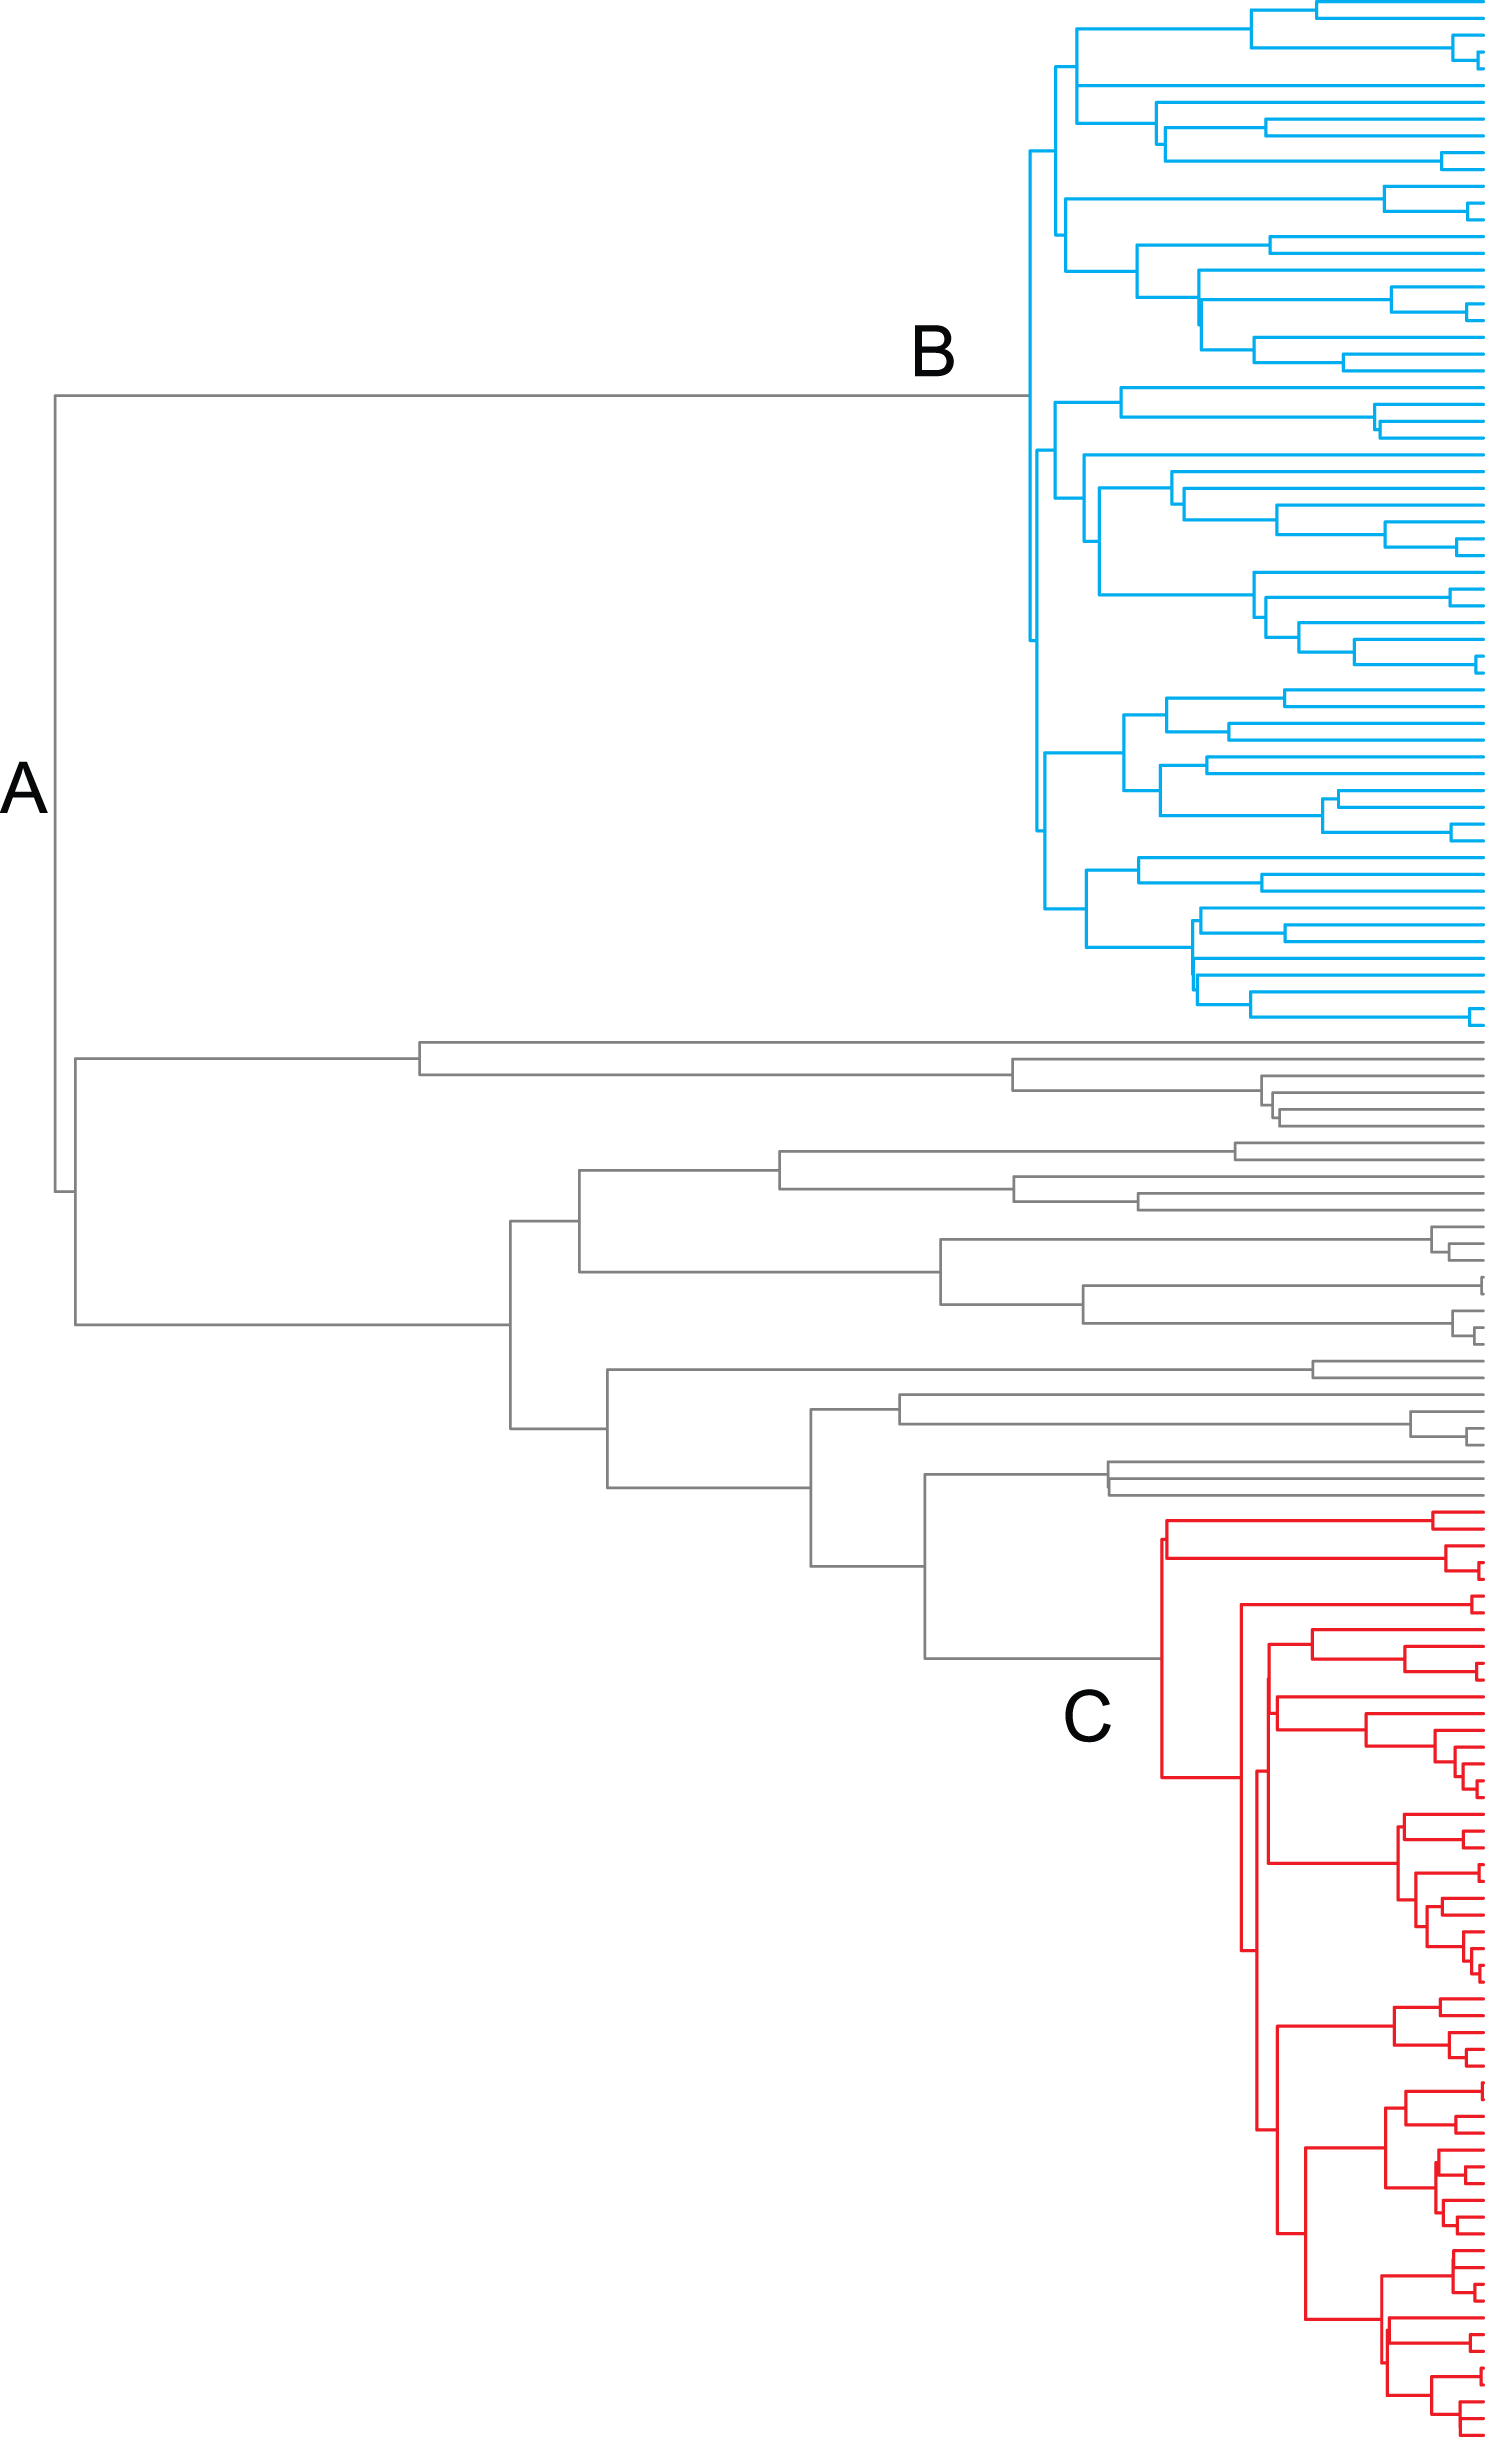
\includegraphics[width=0.3\textwidth]{bamm.png}
\caption{
    Example of tree simulated under mixture of three distinct evolutionary processes.
    (A) Clade diversification under constant-rate ``background'' diversification process with 
    $\lambda = 0.032$ and $\mu = 0$. 
    (B) Shift to new adaptive zone with subsequent diversity-dependent regulation of 
    speciation and diversity-independent extinction 
    (blue branches; $\lambda_0 = 0.395; K = 66; \mu = 0.041$). 
    (C) Another lineage shifts to diversity-dependent speciation regime (red branches; 
    $\lambda_0 = 0.21; K = 97; \mu = 0.012$).
    Text and image from \protect\citet{rabosky2014automatic}}
\end{figure}

\section{Inferring diversification rate shifts}

The BiSSE class of models test whether a character's state is associated
with different diversification rates.
But how do we detect shifts in diversification rates
without character information or without specifying the locations
of rate shifts ahead of time?
The program BAMM \citep[Bayesian Analysis of Macroevolutionary Mixtures][]{rabosky2014automatic}
models time-varying and heterogenous diversification processes on phylogenies (see Figure 3).
The BAMM model assumes that  distinct diversification regimes
 occur across the branches of phylogenetic trees under a compound Poisson process.
 This allows for complex mixtures of time-dependent, diversity-dependent, and constant-rate diversification processes
 through time and among lineages.

Here we will run a BAMM analysis over an example whale phylogeny.
Our goal is to identify the set of diversification rate shifts 
that best fits the data (see Figure 4).
The BAMM model can approximate continuous variation in evolutionary rates
by inferring multiple discrete rate shifts.
\begin{figure}[H]
\centering
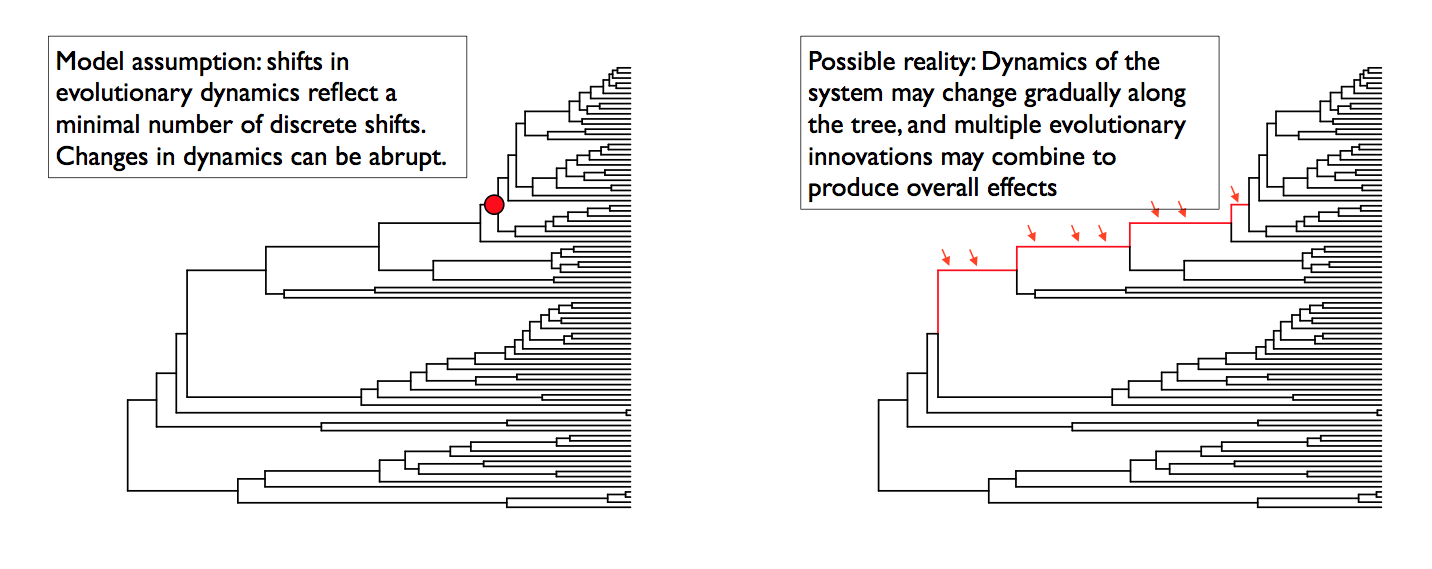
\includegraphics[width=0.6\textwidth]{x_interpret1.png}
\caption{
    The tree on the left depicts the maximum shift credibility configuration identified by BAMM. This is simply the shift configuration sampled during simulation of the posterior with the highest marginal probability, analogous to the ``maximum clade credibility tree'' sampled during a Bayesian phylogenetic analysis (see below). The tree on the right gives an alternative interpretation of the results that would be invisible in the BAMM framework. Here, a relatively minor set of evolutionary shifts combine to produce - over several branches (red) - a major shift in evolutionary dynamics.
    Text and image from \protect\url{http://bamm-project.org/rateshifts.html}}
\end{figure}

\subsection{Setting up a BAMM analysis}

Download the \texttt{whales.tre} and \texttt{template\_diversification.txt}
files from here:
\begin{itemize}
\item \url{http://ib.berkeley.edu/courses/ib200/labs/13/whales.tre}
\item \url{http://ib.berkeley.edu/courses/ib200/labs/13/template\_diversification.txt}
\end{itemize}
Modify the following lines of
\texttt{template\_diversification.txt}:
\begin{code}
treefile = whales.tre
simulatePriorShifts = 0
numberOfGenerations = 100000
mcmcWriteFreq = 1000
eventDataWriteFreq = 1000
printFreq = 100
acceptanceResetFreq = 1000
\end{code}
Run the analysis:
\begin{code}
bamm -c template_diversification.txt
\end{code}

\subsection{Check for MCMC convergence}

We'll use R to check for MCMC convergence and summarize
the output from our BAMM analysis.
Be sure to set your R working directory to the
same directory you ran BAMM in.

First, let's check 
convergence with a quick and dirty plot of
the MCMC log-likelihood trace:
\begin{code}
mcmcout <- read.csv("mcmc_out.txt", header=T)
plot(mcmcout$logLik ~ mcmcout$generation)
\end{code}
Discard the first \%50 of samples as burnin:
\begin{code}
burnstart <- floor(0.5 * nrow(mcmcout))
postburn <- mcmcout[burnstart:nrow(mcmcout), ]
\end{code}
Now calculate the effective sample size (ESS)
for the log-likelihood values
    and for the parameter we are most interested
    in -- the number of diversification rate shifts.
    To calculate ESS we'll use the R package \textbf{coda}, 
    which was mentioned in earlier labs though not required.
    Install it if you need to.
\begin{code}
library(coda)
effectiveSize(postburn$N_shifts)
effectiveSize(postburn$logLik)
\end{code}

\begin{framed}
\noindent
\textbf{Question 3:} \\
Using both the log-likelihood trace plot
and the ESS values, did the MCMC converge?
\end{framed}

\subsection{Summarize the results}

For the sake of time, we are going to go ahead
and summarize our results.
Obviously, if the MCMC has not converged none
of these results should be taken seriously!

We'll use the R package \textbf{BAMMtools} \citep{rabosky2014bammtools}
to summarize the results. First read in data:
\begin{code}
install.packages("BAMMtools")
tree = read.tree("whales.tre")
edata = getEventData(tree, eventdata = "event_data.txt", burnin=0.5)
summary(edata)
\end{code}

\begin{framed}
\noindent
\textbf{Question 4:} \\
What is maximum a posteriori (MAP) number of diversification rate shifts?
\end{framed}

Now let's visualize the mean, model-averaged speciation rates 
along the entire phylogeny:
\begin{code}
plot.bammdata(edata, lwd=2, legend=T)
\end{code}
Looks cool. This averaged over all the 
models (different shift configurations) proportionately
to their posterior distribution.
One clade -- the dolphins -- is inferred to
be undergoing much high speciation rates compared
to the rest of the whales.


What if we want to visualize the individual rate
shift configurations?
Using this we can visualize the credible set of shift configurations over the tree:
\begin{code}
css <- credibleShiftSet(edata, expectedNumberOfShifts=1, threshold=5, set.limit = 0.95)
css$number.distinct
summary(css)
plot.credibleshiftset(css)
\end{code}

\subsection{Caveats}

The BAMM model assumes that
diversification rate shifts do not occur
on the unobserved branches that went extinct.
This means the model assumes some lineages
can effectively predict the future -- if the lineage
will eventually go extinct it cannot undergo a rate shift.
This is highly unrealistic and will bias the calculation of extinction probabilities.
Simulations have shown that rate shifts on
lineages going extinct do not strongly
influence estimates, however the consequences
for empirical data are unknown.
Another approach that solves this
problem is implemented in RevBayes.
The approach used in RevBayes is to make
the diversification rates 
drawn from a discrete (as opposed to continuous)
distribution.
This allows RevBayes 
 to numerically
 integrate over all possible rate categories
 and correctly calculate probabilities.

A forthcoming paper in PNAS has
shown that BAMM analyses can be
highly sensitive to the prior on the 
expected number of rate shifts.
If you use BAMM or other similar models you should
consider experimenting with different priors
and testing whether your results
are robust to different choices on the prior.

\begin{framed}
\noindent
\textbf{Question 5:} \\
How could incorporating fossils into a BAMM analysis
affect the outcome?
\end{framed}

\begin{framed}
\noindent
\textbf{Please email me the following:}
\begin{enumerate}
  \item Your answers to questions 1-5.
\end{enumerate}
\end{framed}

\bibliographystyle{plainnat}
\bibliography{\jobname} 

\end{document}

